\documentclass{report}
\usepackage[utf8]{inputenc}
\usepackage{graphicx}
\usepackage{multirow}

\title{Softwarepraktikum Parallele Numerik}
\date{2019-08-28}
\author{Rebecca, Joshua, Alexander}

\renewcommand{\contentsname}{Inhaltsverzeichnis}

\begin{document}
    \maketitle
        \newpage
    \tableofcontents
    \newpage
    \chapter{Poisson-Gleichung und OpenMP}
    \section{OpenMP und Testtools}
    \subsection{Aufgabe 1}
        \subsubsection{a)}
        Die Reihenfolge in welcher die IDs der Threads ausgegeben werden ist jedes Mal unterschiedlich und ist auch nicht vorherzusagen.
        
        \subsubsection{b)}
        Gemessen wurde auf dem i82sn02. In Table \ref{Table:1b} sind die Messungen dokumentiert. Für die manuelle Parallelisierung wurde atomic verwendet. Diese Messung wurde nach 4 Threads aufgehört da sich die Rechenzeit stark erhöht hat. Für das Parallelisieren mit Reduktion ist das maximales Speedup $ \sim 8 $.\\
        Bei 16 und 32 Threads verschlechtert sich die Beschleunigung im Gegensatz zu 8 Threads bei kleineren N. Das könnte am Overhead der Verarbeitung der Threads liegen.
   \begin{table}     
	\begin{tabular}{|l|l|r|r|r|}
		\hline
		- & Number of Threads & N & Time (s) & Speedup \\
		\hline
		sequential & 1 & 1000 & 0.002 & - \\
		& 1 & $10^{7}$ & 0.239 & - \\
		& 1 & $10^{8}$ & 2.388 & - \\
		& 1 & $10^{9}$ & 23.642 & - \\
		& 1 & $10^{10}$ & 239.508 & - \\
		\hline
		manual & 2 & 1000 & 0.002 & 1 \\
		 & 2 & $10^{7}$ & 0.634 & - \\
		 & 2 & $10^{8}$ & 6.461 & - \\
		 & 2 & $10^{9}$ & 52.989 & - \\
		 & 4 & $10$ & 0.003 & - \\
		 & 4 & $10^{7}$ & 1.214 & - \\
		 & 4 & $10^{8}$ & 13.491 & - \\
		 & 4 & $10^{9}$ & $\sim$ 120 & - \\
		\hline
		reduction & 2 & 1000 & 0.002 & 1 \\
		 & 2 & $10^{7}$ & 0.121 & 1.9 \\
		 & 2 & $10^{8}$ & 1.188 & 2 \\
		 & 2 & $10^{9}$ & 11.845 & 1.9 \\
		 & 2 & $10^{10}$ & 118.204 & 2 \\
		 & 4 & 1000 & 0.003 & - \\
		 & 4 & $10^{7}$ & 0.062 & 3.9 \\
		 & 4 & $10^{8}$ & 0.595 & 4 \\
		 & 4 & $10^{9}$ & 5.959 & 3.9 \\
		 & 4 & $10^{10}$ & 59.183 & 4 \\
		 & 8 & 1000 & 0.003 & - \\
		 & 8 & $ 10^{7} $ & 0.032 & 7.5 \\
		 & 8 & $ 10^{8} $ & 0.299 & 7.9 \\
		 & 8 & $ 10^{9} $ & 2.967 & 7.9 \\
		 & 8 & $10^{10}$ & 29.689 & 8.0 \\
		 & 16 & 1000 & 0.003 & - \\
		 & 16 & $ 10^{7} $ & 0.040 & 5.9 \\
		 & 16 & $ 10^{8} $ & 0.318 & 7.5 \\
		 & 16 & $ 10^{9} $ & 3.028 & 7,8 \\
		 & 16 & $10^{10}$ & 29.674 & 8.1\\
		 & 32 & 1000 & 0.004 & - \\
		 & 32 & $ 10^{7} $ & 0.037 & 6.4 \\
		 & 32 & $ 10^{8} $ & 0.305 & 7,8 \\
		 & 32 & $ 10^{9} $ & 2.987 & 7.9 \\
		 & 32 & $10^{10}$ & 29.551 & 8.1 \\
		\hline
	\end{tabular}
	\caption{OpenMP Parallelisierung mit verschiedenen Threadanzahlen und Synchronisationsmechanismen}
	\label{Table:1b}
\end{table}
	\newpage
        \subsubsection{c)}
        
        Die Messbedingungen waren gleich wie im Aufgabenteil b). Die Werte für das Speedup unterscheiden sich nicht groß von den oben gemessenen. Die Messungen sind in Table  \ref{Table:1c}.\\
        \begin{table}
        \begin{tabular}{|l|r|r|r|}
        	\hline
        	 Auflösung N & No. Threads &  Time (s) & Speedup \\
        	 	\hline
        	 1000& 1 &  4.411 & - \\
        	 1000& 2 &  2.228 & 1.980 \\
        	 1000& 4 &  1.122 & 3.931 \\
        	 1000& 8 &  0.563 & 7.835\\
        	 1000& 16 &  0.567 & 7.780 \\
        	\hline
        	2000& 1 & 17.625 & - \\
        	2000& 2 &  8.896& 1.981 \\
        	2000& 4 &  4.493& 3.923 \\
        	2000& 8 &  2.254& 7.819 \\
        	2000& 16 &  2.248& 7.840 \\
        	\hline
        	4000& 1 & 71.761 & - \\
        	4000& 2 &  35.559 & 2.010 \\
        	4000& 4 &  17.952& 3.997 \\
        	4000& 8 &  8.978 & 7.991\\
        	4000& 16 &  8.980 & 7.991 \\
        	\hline
        	5000& 1 &  110.143 & - \\
        	5000& 2 &  55.564 & 1.982 \\
        	5000& 4 &  27.951 & 3.94 \\
        	5000& 8 &  13.995 & 7.870 \\
        	5000& 16 &  14.020 & 7.856\\
        	\hline
        \end{tabular}
        \caption{Messungen zu Aufgabe 1c}
         \label{Table:1c}
        \end{table}
	\begin{center}
		
\includegraphics[width=0.6\linewidth]{Aufgaben-Ressourcen/normal-1000.jpg}	
	\end{center}

	\begin{center}
		
\includegraphics[width=0.4\linewidth]{Aufgaben-Ressourcen/critical-1000.jpg}\quad
\includegraphics[width=0.4\linewidth]{Aufgaben-Ressourcen/critical-1000-1000.jpg}
		\\[\baselineskip]
		\includegraphics[width=0.4\linewidth]{Aufgaben-Ressourcen/critical-10000-1000.jpg}\quad\includegraphics[width=0.4\linewidth]{Aufgaben-Ressourcen/critical-10000-1000.jpg}
	\end{center}


    \subsection{Aufgabe 2}
    	\subsubsection{a)}
		\begin{enumerate}
			\item Example: \\
				Es besteht eine Race-Condition auf dem Array a über Index i,
				bei ungünstiger Ausführungsreihenfolge der Threads kann es dazu kommen,
				das a[i] durch einen Thread geschrieben wird und von einem anderen Thread versucht wird, darauf in der nachfolgenden Anweisung lesend zuzugreifen.
				Um dieses Problem zu lösen können zwei for-Schleifen verwendet werden.
				Eine schreibt alle Werte in Array a und die zweite schreibt alle Werte unter Zugriff auf Array a in Array b. 
				Beide Schleifen werden jeweils getrennt parallelisiert.
			\item Example: \\
				Threads exisiteren hier in der gesamten parallelen Region.
				Das nowait-Statement der ersten parallelisierten For-Schleife bewirkt, dass Threads bereits die nächste parallelisierte Schleife bearbeiten können, wenn sie ihren Teil der ersten Schleife fertig verarbeitet haben.
				Dies führt zu einer Race-Condition auf das Array a mit Index i, ähnlich zu Example 1.
				Mit dem entfernen des nowait-Statements der ersten for-Schleife warten alle Threads wieder auf die implizite Barriere bis alle Threads fertig sind und es kann Problemlos auf die geschriebenen Werte in Array a zugegriffen werden.
			\item Example: \\
				Hier ist die Variable x zunächst global definiert und wird somit implizit zwischen den Threads geshared. 
				Somit besteht eine Race-Condition auf x da die Threads unabhängig voneinander sowohl lesend als auch schreibend auf x zugreifen.
				Indem man x explizit als private deklariert, erhält jeder Thread seine eigene Kopie der Variable und es besteht keine Race-Condition mehr.
			\item Example: \\
				f ist global definiert und wird durch jeden Thread private gesetzt. 
				Allerdings erhält jeder Thread eine uninitialiserte Kopie der Variable f, was bedeutet das dass initialisieren mit dem Wert 2 vor der Schleife nur für den Master-Thread sichtbar ist.
				Um diese Initialiserung auch für alle übrigen Threads sichtbar zu machen, ist es erforderlich, f mittels firstprivate zu deklarieren.
				Des weiteren wird der Wert von x nicht aus der parallelen Region wieder rausgeschrieben, sondern gelöscht. 
				Wodurch der zuletzt geschriebene Wert innerhalb der parallelen Region in x nach außen hin nicht sichtbar ist.
				Um deses Verhalten zu erreichen, muss x als lastprivate deklariert werden.
			\item Example: \\
				Hier besteht eine Race-Condition auf die Variable sum. 
				Da mehrere Threads versuchen hier den alten Wert von Sum zu lesen, den i-ten Wert aus b ausfzuaddieren und damit sum wieder zu überschreiben, ist nicht garantiert, dass sum am Ende den korrekten Wert enthält.
				Indem man das auslesen, aufaddieren und zuweisen mittels critical-Konstrukt schützt, ist garantiert das immer nur ein Thread den Wert überschreiben kann.
				Allerdings ist die gesamte Schleife dann gleichbedeutend mit einer Sequenziellen Ausführung.
		\end{enumerate}

		\subsubsection{b)}
			Werden Matrizen in C zeilenweise im Speicher hinterlegt, ist es zur optimalen Ausnutzung von Caching-Effekten ideal, wenn auch zeilenweise über Einträge der Matrix iteriert wird.
			Dadurch läd der Prozessor bei einem Cache-miss auf einen Eintrag nicht nur den einzelnen Eintrag in den Cache, sondern direkt mehrere nachfolgende Einträge, was weniger Zugriffe auf den RAM zu folge hat und somit insgesamt die Performance verbessert.
			Wird jedoch spaltenweise über eine Matrix iteriert, müssen für einen Zugriff auf das (i+1)-te Element alle n-Einträge nach i ausgelassen werden. 
			Bei entsprechend großen Matrizen werden die mit in den Cache geladenen Elemente garnicht benötigt.
			Jeder Zugriff entspricht somit einem Cache-miss, was wiederum einen Speicherzugriff zur folge hat und somit die gesamte Performance negative beeinflusst.
			
			Der klassische IJK-Algorithmus zur Matrixmultiplikation iteriert in der inneren K-Schleife für die rechte Matrix B für jede Addition+Multiplikation über die Spalten.
			Zum besseren Ausnutzen der Cache-Effekte kann durch vertauschen der zwei Schleifen J und K, auch bekannt als IKJ-Optimierung, eine Verbesserung der Performance erzielt werden.
			So wird in der inneren J-Schleife nur über die Spalten aus B und C iterriert und die K-Schleife iteriert über die Spalten in A.

			Da der einzelne Eintrag in A der inneren Schleife invariant ist, kann dieser zudem aus der Schleife herausgezogen und in einer tempäreren Variable gespeichert werden. \\
			Die Messungen und Speedup für verschiedene Threadanzahlen sieht man in Table \ref{Table:2b}.

			\begin{table}
			\begin{tabular}{|l|p{1cm}|p{1cm}|p{1cm}|p{1.5cm}|r|r|r|r|}
				\hline
			\multirow{2}{*}{Mode} & \multirow{2}{*}{N} & \multirow{2}{*}{Seq} & \multicolumn{2}{|c|}{2 Threads} & \multicolumn{2}{|c|}{4 Threads} & \multicolumn{2}{|c|}{16 Threads} \\
				& & & Zeit & Speedup & Zeit & Speedup & Zeit & Speedup \\
				\hline
				% Methode | Problemgröße | Seq Laufzeit | 2 Threads      | 4 Threads      | 16 Threads     |
				%		  |              |              | Time | Speedup | Time | Speedup | Time | Speedup |
				gcc - IJK & 10 & 		   0.0040  &     0.0040  &  1.00&      0.0040   & 1.00 &      0.0040  &  1.00\\
				
				gcc - IJK & 100 &           0.0190  &     0.0140  &  1.36&      0.0090   & 2.11&      0.0070  & 2.71\\
				
				gcc - IJK & 1000 &          8.8990  &     4.5550  &  1.95&        2.3770   & 3.74&       0.7240  & 12.29\\
				\hline
				gcc - IKJ  & 10 & 			0.0040  & 	 0.0040  & 1.00 & 	  0.0040  &  1.00&			0.0040 & 1.00\\
				
				gcc - IKJ & 100 &			0.0166  &     0.0122  &  1.36&		 0.0088  & 1.89&         0.0060  & 2.77\\
				
				gcc - IKJ & 1000 & 			7.3744  & 	 7.8727  & 0.94& 	  3.8862 & 1.90&         1.6994  & 4.34\\
				\hline
				gcc - ... +Inv & 10 &      0.0030  &     0.0030  & 1.00&       0.0030  & 1.00&        0.0040  & 0.75\\
				gcc - ... +Inv & 100 &	    0.0160  &     0.0116  & 1.38&       0.0090  & 1.78&			0.0056 & 2.86\\
				gcc - ... +Inv & 1000 & 	6.0300  &	3.1956  & 1.89&			1.7114 & 3.52&		0.5086 & 11.86\\
				\hline
				gcc - ... +O2 & 10 &  0.0040  &     0.0036  &  1.11&      0.0040   & 1.00&      0.0042  &  0.95\\
				 
				gcc - ... +O2 & 100 & 0.0060  &	  0.0062  &  0.97 &		0.0050  & 1.20 &        0.0050  &  1.2\\
				
				gcc - ... +O2 & 1000 & 6.0412  & 	3.1912 & 1.89 &       1.7174  & 3.52 &		  0.5078 & 11.9\\
				\hline
			\end{tabular}
			\caption{Verschiedene Varianten der Matrixmultiplikation}
			\label{Table:2b}
		\end{table}
		\subsubsection{c)}
			Die Arbeitspakete pro Thread werden statisch vergeben. 
			Die Berechnung der Mandelbrotmenge ist jedoch nur für einen bestimmten Bild Bereich besonders Berechnungsintensiv. 
			Threads welche diese Bereiche berechnen sollen, müssen mehr Aufwand betreiben im vergleich zu den anderen Threads, wodurch diese insgesamt länge benötigen.
			Die anderen Threads werden kaum ausgelastet und die gesamte Parallelisierung ist ineffizient.
			Durch dynmisches Scheduling werden die Arbeitspakete erst an Threads verteilt, wenn diese keine Aufgabe haben oder eine bereits beendet haben.
			Dies führt zu einer optimaleren Verteilung der Arbeitslast und insgesamt schnelleren Berechnung des Gesamtproblems, da alle Threads möglichst gleich viel Arbeiten. Siehe Table \ref{Table:2c}.
	
			\begin{table}
				\begin{tabular}{|p{1.5cm}|p{2cm}|p{1cm}|p{1cm}|p{1cm}|p{1cm}|p{1cm}|p{1cm}|p{1cm}|}
					\hline
					Mode & N, It., Chunk & Seq. & 2 Threads & S.Up & 4 Threads & S.Up & 8 Threads & S.Up \\
					\hline
					static & 2000, 500, - & 8.528  & 6.188  & 1.38 & 5.453  & 1.56 & 3.908  & 2.18\\
					static & 4000, 500, - & 34.080  & 24.881  & 1.37 & 22.193  & 1.54 & 15.061  & 2.26 \\
					static & 8000, 500, - & 135.882  & 98.576  & 1.38 & 86.120  & 1.56  & 60.522  & 2.25 \\
					\hline
					dynamic & 2000, 500, 1 & 8.524  & 4.375  & 1.95 & 2.284 & 3.73 & 1.216 & 7.01 \\
					dynamic & 4000, 500, 1 & 33.955  & 17.016 & 2.00 & 8.600 & 3.95 & 4.803 & 7.07 \\
					dynamic & 8000, 500, 1 & 135.966  & 67.987 & 2.00 & 34.344 & 3.96 & 19.110 & 7.11 \\
					\hline
				\end{tabular}
				\caption{Auswirkung der Chunk-Size auf die Performance}
				\label{Table:2c}
			\end{table}
			
			Veränderungen in der Chunk-Size beim Scheduling wirken sich in diesem Fall nicht auf die Performance aus. Dies sieht man in Table \ref{Table:2c2}.
			
			\begin{table}
				\begin{tabular}{|r|r|r|r|r|r|}
					\hline
					Chunk & N & Seq. & 2 Threads & 4 Threads & 8 Threads \\
					\hline
					1 & 8000 & 135.966 & 67.987  & 34.569  & 19.042  \\
					\hline
					2 & 8000 & - & 68.069 & 34.569  & 19.049  \\
					\hline
					4 & 8000 & - & 69.999  & 34.471  & 19.049  \\
					\hline
					8 & 8000 & - & 68.027  & 34.533  & 19.096  \\
					\hline
					16 & 8000 & - & 67.996  & 34.892  & 19.134  \\
					\hline
				\end{tabular}
				\caption{Stabile Performance unabhängig von der Chunk-Size}
				\label{Table:2c2}
			\end{table}

\section{Parallelisierung}
    \subsection{Aufgabe 3}
    
        \subsubsection{a)}
        P(x): Anzahl auszuführender Operationen auf x Prozessoren.\\
        T(x): Ausführungszeit auf x Prozessoren.\\
        
        \textbf{Speedup}:  $S(n) = T(1)/T(n) $. \\ Der Zusammenhang zwischen serieller und paralleler Ausführungszeit eines Programmes. Der Wertebereich ist $ 1 \leq S(n) \leq n $ .\\
        
        \textbf{Effizienz}: Die Effizienz $ E(n) = S(n)/n $ gibt die relative Verbesserung der Verarbeitungsgeschwindigkeit an.\\
        
        \textbf{Auslastung}: $ R(n)/(n*T(n)) $. Gibt an, wie viele Operationen (Tasks) jeder Prozessor im Durchschnitt pro Zeiteinheit ausgeführt hat.\\
        
        \textbf{Mehraufwand}: $ R(n) = P(n)/P(1) $. Beschreibt den bei einem Multiprozessorsystem erforderlichen Mehraufwand für die Organisation, Synchronisation und Kommunikation der Prozessoren.\\
        
        \subsubsection{b)}
        Race-Conditions: Wenn zwei Threads unabhängig voneinander auf eine Ressource lesend oder auch schreibend zugreiffen können, 
        spricht man von einer Race-Condition. Hierbei kann es bspw. beim Zugriff auf Variablen bei ungünstiger Ausführungszeiten
        dazu kommen, dass am Ende der Berechnungen ein falscher Wert in der Variable enthalten ist, als wenn die Berechnung sequentiell 
        ausgeführt worden wäre.
        Um eine Race-Condition zu vermeiden, können die kritischen Abschnitte in der Art und weise gesichert werden, das immer nur ein 
        Thread gleichzeitig innerhalb des kritischen Abschnitts sein darf.

        In diesem Zusammenhang kann es auch zu Deadlocks, Lifelocks oder auch Starvation kommen. 
        \subsubsection{c)}
        \begin{table}
        \begin{tabular}{|p{4cm}|p{3cm}|p{3cm}|p{3cm}|}
        	\hline
        	- & GPUs & CPUs & FPGAs \\
        	\hline
        	Energieeffizienz & Gut & Mittel & Gut  \\
        	\hline
        	Anwenderfreundlichkeit & \begin{itemize}
        		\item Braucht Einarbeitungszeit.
        		\item Es gibt Bibliotheken.
        	\end{itemize} & 
        \begin{itemize}
        	\item Am einfachsten zu programmieren.
        	\item Viele Bibliotheken vorhanden. 
        	\item Kurze Compilierzeit.
        \end{itemize}  & \begin{itemize}
        \item Aufwändig zu programmieren.
        \item Lange Compilierzeit.
        \item Wenig Bibliotheken.
    \end{itemize}  \\
        	\hline
        \end{tabular}
        \caption{Bewertung verschiedener Programmierplattformen}
        \label{Table:3c}
        \end{table}
    
    In diesem Praktikum verwenden wir CPUs und GPUs da sie universeller einsetzbar sind als FPGAs und die Programmierung deutlich leichter ist. Eine ausführlichere Bewertung ist in Table \ref{Table:3c} aufgeführt.


    \subsection{Aufgabe 4}
	\begin{figure}
		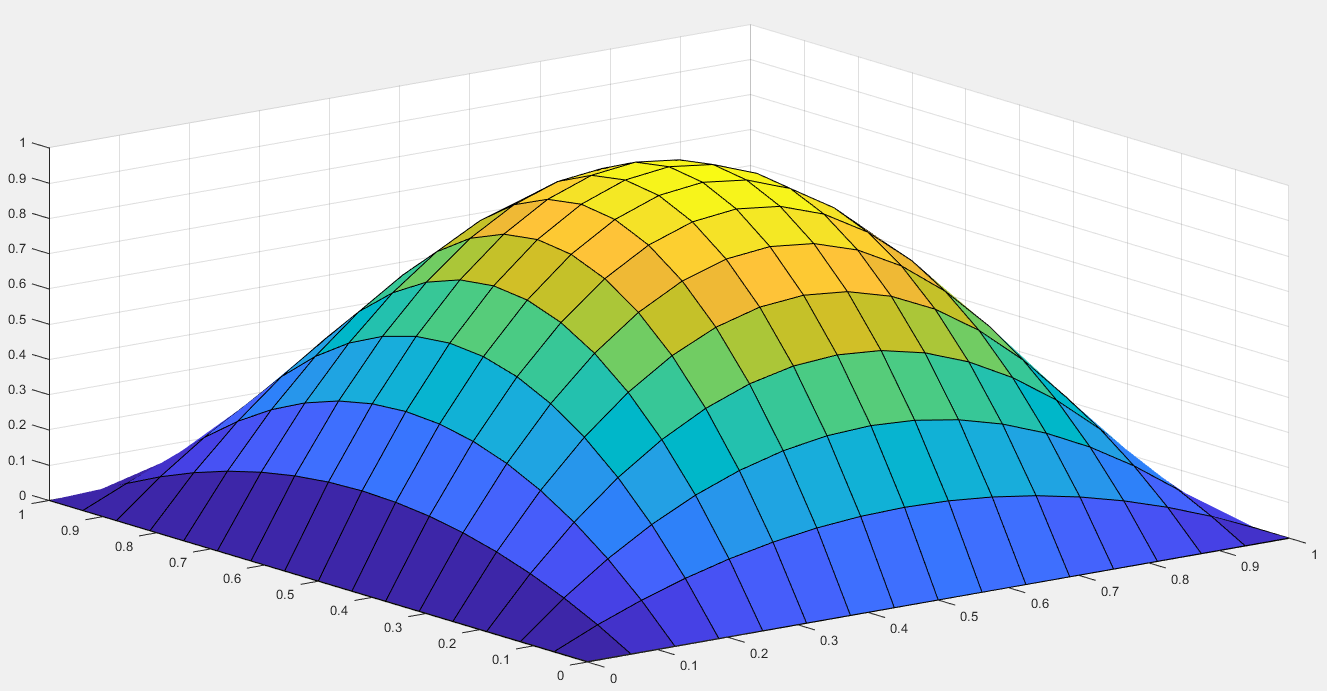
\includegraphics[width=\linewidth]{Aufgaben-Ressourcen/A4L4.png}
		\caption{l=4; h=1/16;}
		\label{A4L4}
	\end{figure}
\begin{figure}
		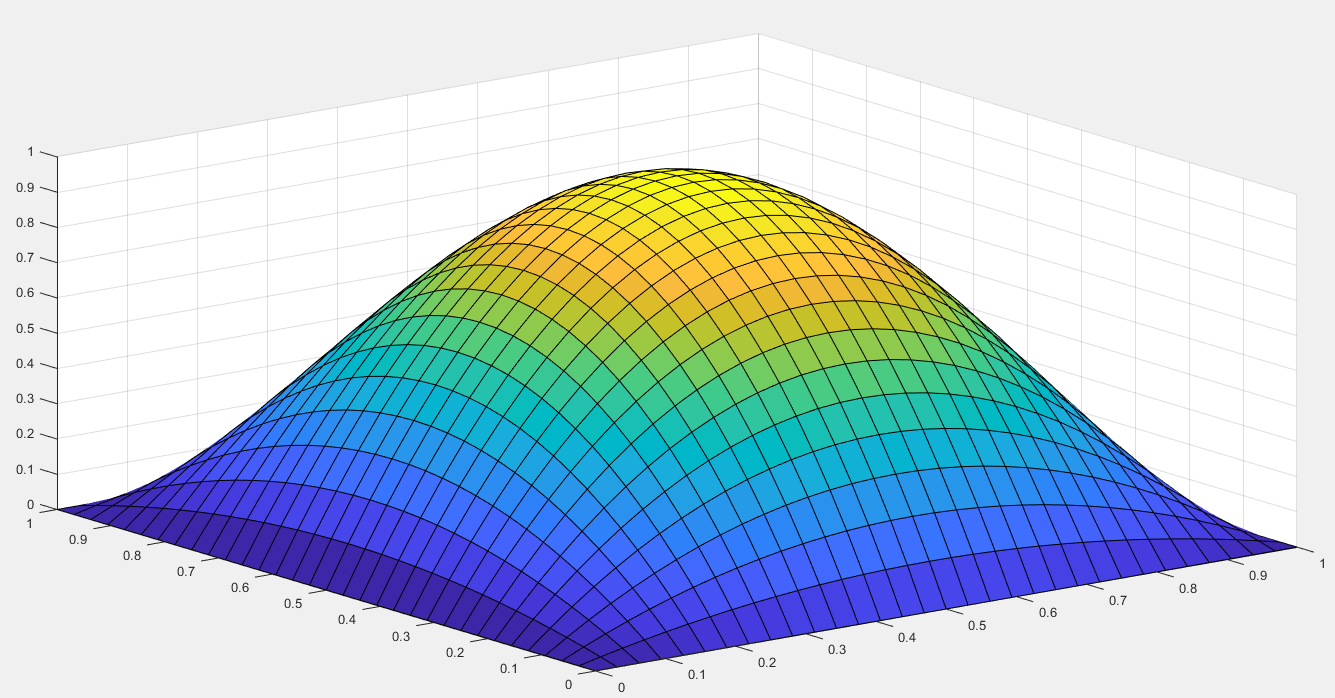
\includegraphics[width=\linewidth]{Aufgaben-Ressourcen/A4L5.png} 
		\caption{l=5; h=1/32;}
		\label{A4L5}
	\end{figure}
	\begin{figure}
		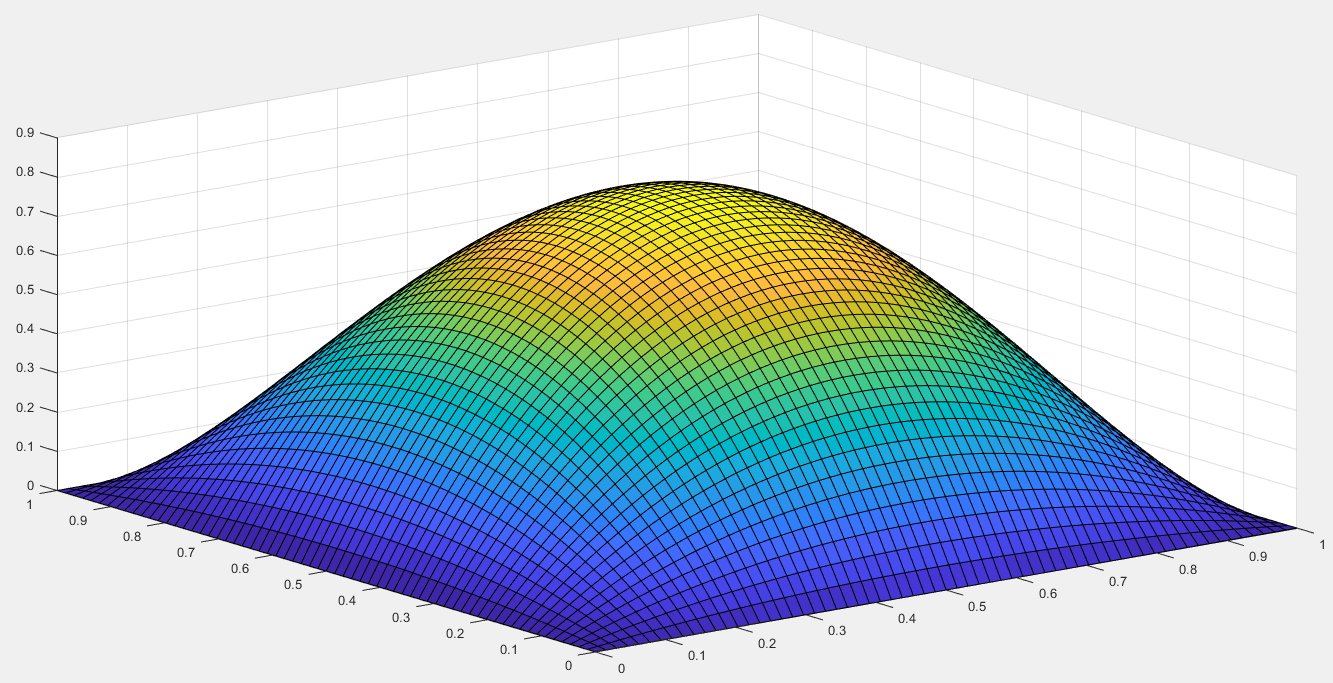
\includegraphics[width=\linewidth]{Aufgaben-Ressourcen/A4L6.png} 
		\caption{l=6; h=1/64;}
		\label{A4L6}
	\end{figure}


	\subsubsection{a)}
Alle Programmdurchläufe für die Messungen hatten eine Fehlerschranke von 0.000001. Die Laufzeiten bei verschiedenen l und daraus resultierenden h Werten sieht man in Table \ref{Table:4a}.
\begin{table}
\begin{tabular}{|l|l|r|r|}
		\hline
		- & l=4; h=1/16 & l=5; h=1/32 & l=6; h=1/64\\
		\hline
		& 0.050s & 1.429s & 37.296s \\
		& 0.041s & 1.426s & 37.014s  \\
		& 0.040s & 1.392s & 37.061s \\
		& 0.037s & 1.428s & 37.416s  \\
		& 0.051s & 1.424s & 37.295s  \\
		& =0.044s & =1.420s & =37.216s  \\
		\hline

	\end{tabular}
	\caption{Laufzeiten mit verschiedenen l-Werten}
	\label{Table:4a}
\end{table}
	\newline Diese Lösungswerte in Figure \ref{A4L4}, \ref{A4L5} und \ref{A4L6} ergeben sich mit l=4,5,6;  \newline
	
	\subsubsection{b)}
	Die Schleifenabläufe sind direkt voneinander abhängig und müssen in Reihenfolge ablaufen. Die naive Parallelisierung liefert keine korrekten Ergebnisse. Alternativ könnte man mit einer naiven Parallelisierung auch Parallelisierung der beiden inneren Summen meinen. Diese hätte zur Folge, dass man nur bis zu maximal vier parallele Threads hat, welche jeweils nur einen Wert aufaddieren.
	\subsubsection{c)}
		Methodik: Es gibt verschiedene Wege der effizienteren Parallelisierung der Werte. Man kann die zu berechnenden Werte zeilen- oder spaltenweise in Gruppen einteilen, sowie auch in einem Schachbrettmuster. Dann berechnet man die verschiedenen Gruppen parallel. Dies wird umgangssprachlich ''Rot-Schwarz'' genannt und konvergiert zum korrekten Ergebnis. Eine andere Variante der Berechnung ist die sogenannte ''Wavefront''. Dabei werden die Werte diagonal ausgerechnet. Dadurch entsteht eine ungeleiche Last über die Ausführungszeit, welche jedoch ausgeglichen werden kann, indem man die Matrix zusätzlich in Blöcke einteilt. Den Vergleich zwischen der sequentiellen und parallelisierten Version sieht man in Table \ref{Table:4c}.
		\begin{table}
		\begin{tabular}{|l|l|r|r|r|}
				\hline
				&Laufzeit(sequentiell) &Laufzeit(parallel) & SpeedUp & Efficiency\\
			\hline
			l=4; h=1/16 & 0.044s & 0.242s & 0.182 & 0.004 \\
			l=5; h=1/32 & 1.420s & 1.154s & 1.231 & 0.026 \\
				l=6; h=1/64 & 37.216s & 26.884s & 1.384 & 0.029 \\
				\hline

		\end{tabular}
	\caption{Laufzeiten und Speedup des parallelisierten Gauß-Seidel-Verfahren}
	\label{Table:4c}
		\end{table}

\section{Partielle Differentialgleichungen}
    \subsection{Aufgabe 5}
	\begin{figure}
		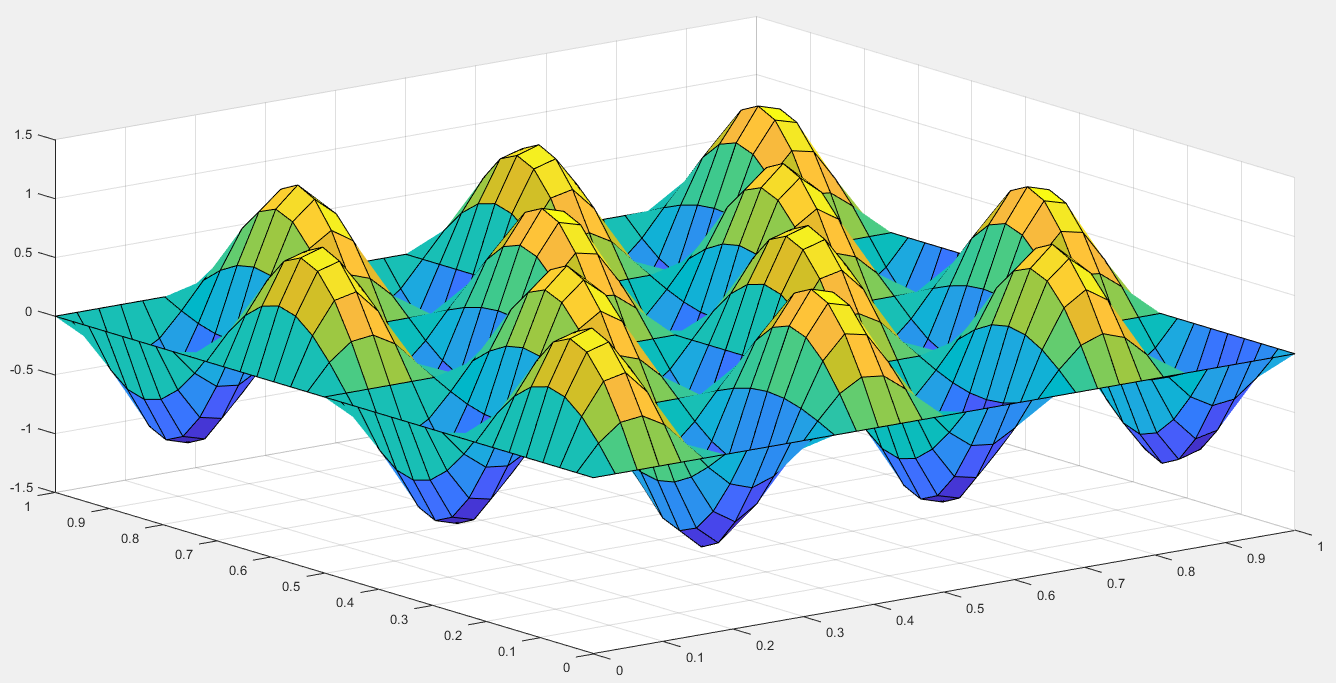
\includegraphics[width=\linewidth]{Aufgaben-Ressourcen/A5L5M3N2.png} 
		\caption{l=5; h=1/32;}
		\label{A5L5}
	\end{figure}
	\begin{figure}
		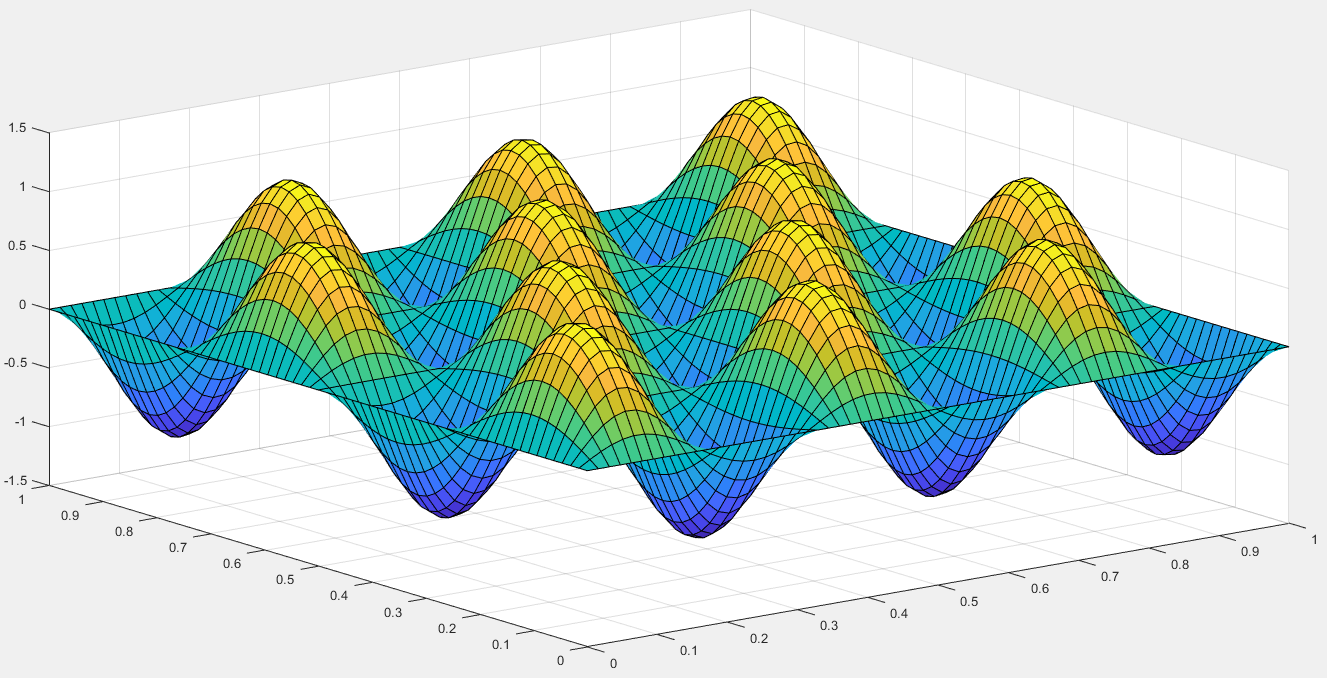
\includegraphics[width=\linewidth]{Aufgaben-Ressourcen/A5L6M3N2.png} 
		\caption{l=6; h=1/64;}
		\label{A5L6}
	\end{figure}
	\begin{figure}
		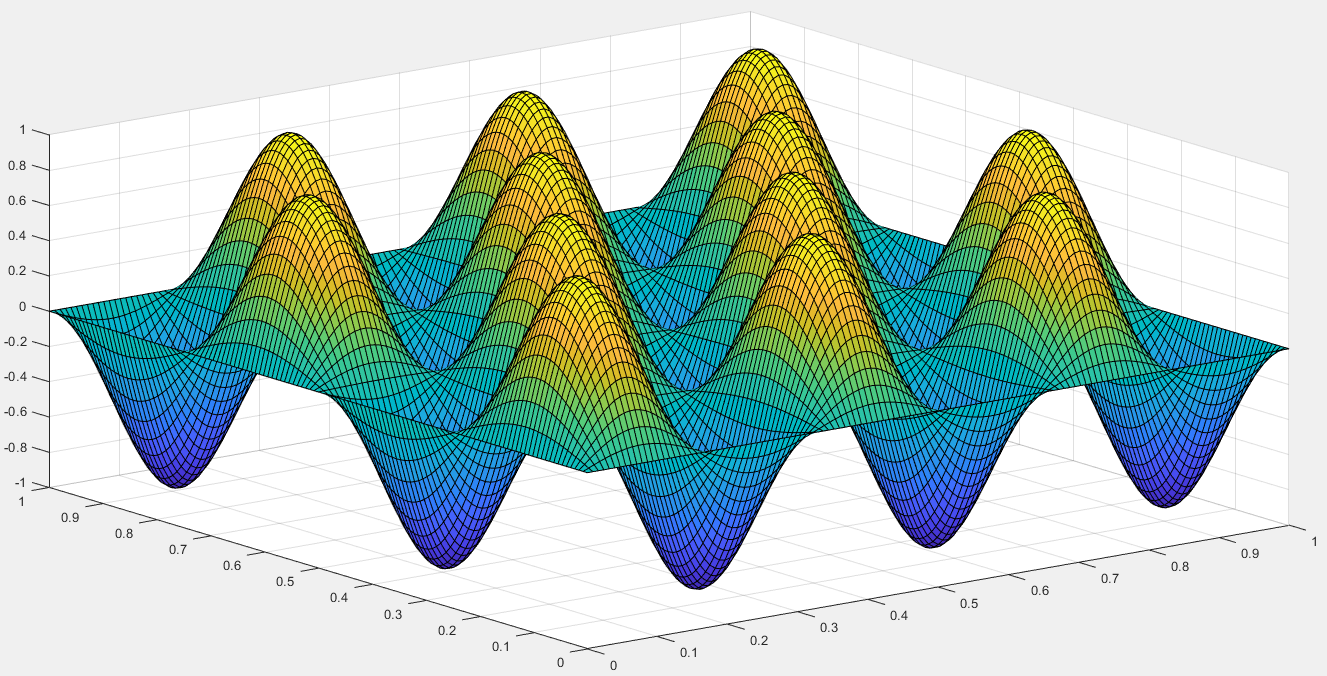
\includegraphics[width=\linewidth]{Aufgaben-Ressourcen/A5L7M3N2.png}
		\caption{l=7; h=1/128;}
		\label{A5L7}
	\end{figure}
	\subsubsection{a)}
	f(x,y) muss stetig definiert sein auf $\Omega$ \newline
	$\Gamma$ ist der Rand von $\Omega$ und lipschitzstetig  \newline
	L\"{o}sung u(x,y) muss zweifach differenzierbar sein 
	\subsubsection{b)}
	f(x,y) = ($N^2$ + $M^2$)*4*$\pi^2$*sin(2*M*$\pi$*x)*sin(2*N*$\pi$*y)
	\subsubsection{c)}
	Es handelt sich um eine h-FEM.  \newline
	Die Lösungswerte in Figure \ref{A5L5}, \ref{A5L6} und \ref{A5L7} ergrben sich mit M=3; N=2; l=5,6,7;  \newline


\subsection{Aufgabe 6}
\begin{figure}
	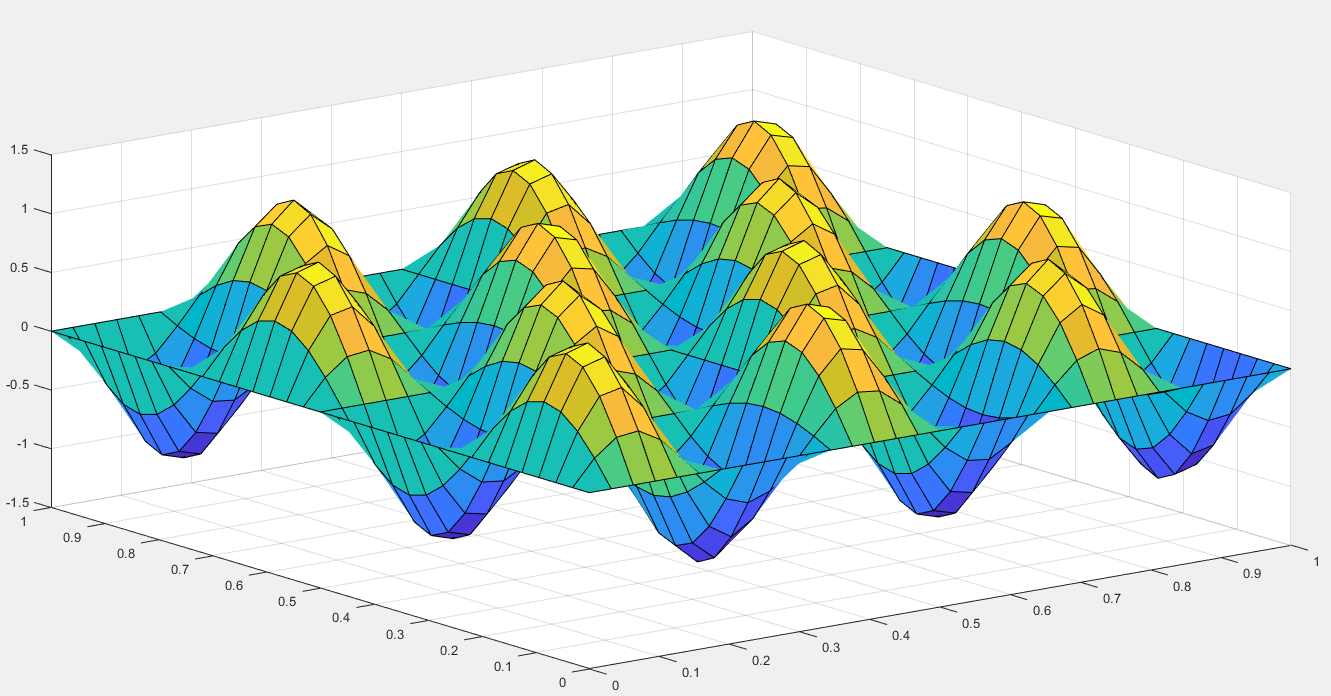
\includegraphics[width=\linewidth]{Aufgaben-Ressourcen/A6L5M3N2.png} 
		\caption{GMRES; l=5; h=1/32;}
		\label{A6L5}
\end{figure}
\begin{figure}
	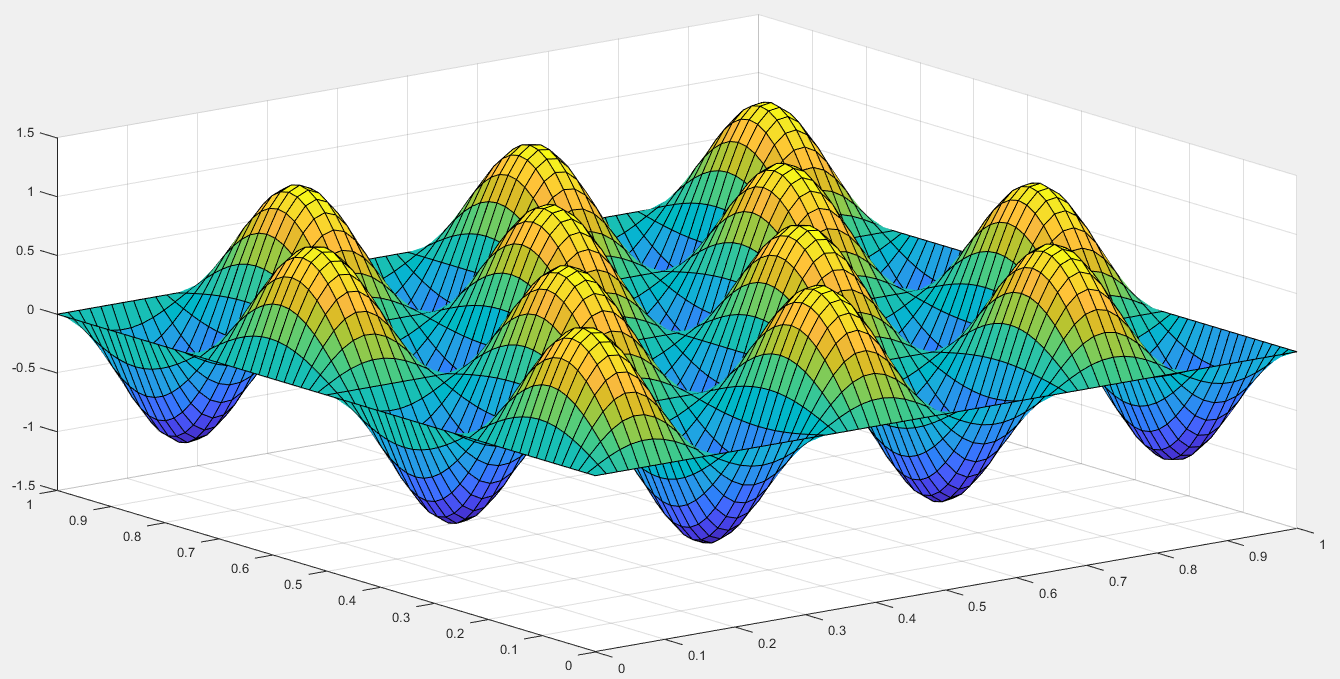
\includegraphics[width=\linewidth]{Aufgaben-Ressourcen/A6L6M3N2.png} 
		\caption{GMRES; l=6; h=1/64;}
		\label{A6L6}
\end{figure}
\begin{figure}
	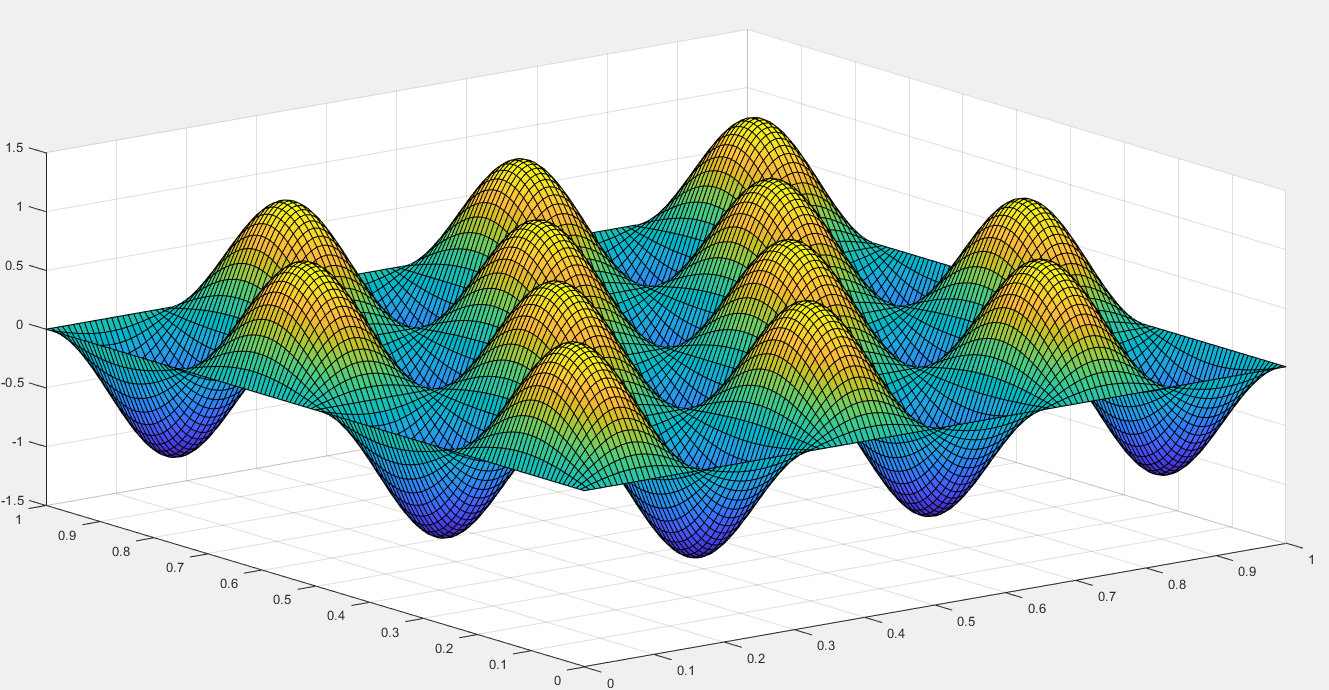
\includegraphics[width=\linewidth]{Aufgaben-Ressourcen/A6L7M3N2.png}
		\caption{GMRES; l=7; h=1/128;}
		\label{A6L7}
\end{figure}
	\subsubsection{a)}
	Liste: CG Verfahren; PCG-Verfahren; Verfahren der minimalen Risiduen(GMRES); GCR-Verfahren; Arnoldi-Verfahren; FOM, ORTHORES;\newline
	Das Gleichungssystem ist dünnbesetzt und alle Krylow-Unterraumverfahren sind gut geeignet f\"{u}r d\"{u}nnvesetzte Gleichungssysteme.
	Diese Lösungswerte in Figure \ref{A6L5}, \ref{A6L6} und \ref{A6L7} ergeben sich mit der Gleichung aus Aufgabe 5 und M=3; N=2; l=5,6,7;  \newline

	\subsubsection{b)}
	Die Verwendung des Residuums als Abrruchbedingung ist eventuell problematisch, da man dadurch in jedem Schleifendurchlauf einen Lösungsvektor $x^k$ berechnen muss. Man kann sich eine feste Anzahl von Iterationen setzen, allerdings hat man dann keine garantierte Genauigkeit. Außerdem kann man das Residuum mit weniger Rechenaufwand in jeder Iteration abschätzen und diesen Schätzwert als Abbruchbedingung nutzen. Auch diese Vorgehensweise hat keine garantierte Genauigkeit, da die Schätzgenauigkeit variiert. Im Zuge des Praktikums haben wir bis jetzt nur eine stabile Version mit abgeschätztem Residuum implementiert(gmres.c). Die Version mit dem Residuum als Abbruchbedingung funktioniert nicht verlässlich(gmresResiduum.c).
	\subsubsection{c)}
Die Efficiency ist bei jedem Vergleich zwischen Aufgabe 6 und Aufgabe 5c gleich dem Speedup, da die Anzahl N der Kerne auf denen das Programm läuft nicht variiert. Der Speedup ist in Table \ref{Table:6c} dokumentiert.\\
\begin{table}
\begin{tabular}{|l|l|r|r|}
		\hline
		- & Aufgabe 5(s) & Aufgabe 6(s) & Speedup\\
		\hline
		l=5; h=1/32 &  +1.450 & +0.028 & 56.96 \\
		& +1.420 & +0.021 &    \\
		& +1.371 & +0.026 &    \\
		& +1.475 & +0.026 &    \\
		& +1.408 & +0.026 &   \\
		&=1.424 & =0.025  & \\
		\hline
		l=6; h=1/64 &  +15.427 & +0.140 & 98.488 \\
		& +12.546 & +0.148 &    \\
		& +12.561 & +0.089 &    \\
		& +12.766 & +0.142 &    \\
		& +13.081 & +0.155 &   \\
		&=13.276 & =0.135  & \\
		\hline
		l=7; h=1/128 &  +107.183 & +1.289 & 81.113 \\
		& +105.581 & +1.188 &    \\
		& +104.562 & +1.175 &    \\
		& +105.834 & +1.703 &    \\
		& +104.077 & +1.148 &   \\
		&=105.447 & =1.300  & \\
		\hline
	\end{tabular}
	\caption{Laufzeiten und Speedup des GMRES gegenüber dem parallelisierten Gauß-Seidel-Verfahren}
	\label{Table:6c}
\end{table}
Einsatz eines Vorkonditionierers: Der Einsatz ist unsinnvoll, da wir bereits eine d\"{u}nn besetzte Matrix gegeben haben. Falls die Matrix anders besetzt wäre, könnte ein Vorkonditionierer von Nutzen sein.
	\subsubsection{d)}
MFEM; deal.II; libMesh; JuliaFEM; FEniCS; Hermes Project;...\newline
Liste weiterer FEM Packages/Libraries: https://en.wikipedia.org/wiki/List\_of\_finite\_element\_software\_packages \newline
Fast alle sind Open Source und kostenlos nutzbar. "Hermes Project" scheint zum Beispiel eine leicht nutzbare C/C++ Bibliothek.

\newpage

\chapter{Partielle Differentialgleichungen und Cuda}
\section{Cuda}
\subsection{Aufgabe 1}

Es gibt sehr viele Eigenschaften die man auslesen kann. Hier sind mögliche Ausgaben: \\

Number of Devices: 2\\
Device Number:                0\\
Device Name:                  Tesla K80\\
Memory Clock Rate (KHz):      2505000\\
Memory Bus Width (bits):      384\\
Global Memory size (bytes):   11996954624\\
Device Number:                1\\
Device Name:                  Tesla K80\\
Memory Clock Rate (KHz):      2505000\\
Memory Bus Width (bits):      384\\
Global Memory size (bytes):   11996954624\\

\subsection{Aufgabe 2}

\paragraph{Arraygröße} Bei kleinen Arrays ist die Transferrate auf der GPU nicht besser als auf der CPU. Das ändert sich aber mit wachsender Arraygröße, denn dann ist die Rate "Device to Device" deutlich besser als "Host to Host".
Hier wurde mit nvprof gemessen. Siehe Table \ref{Table:2_2Groesse}.

\begin{table}
	\begin{tabular}{|l|l|l|l|l|}
		\hline
		N         & Device to Host     & Host to Device     & Device to Device     & Host to Host      \\ \hline \hline
		10			& 2.1120us & 2.0160us &  3.7440us & 3.000us \\ \hline
		100			& 2.3360us & 2.0800us  & 3.8400us & 4.000us\\ \hline
		1000	& 2.6880us & 2.5280us & 3.5200us & 3.000us \\ \hline 
		10000     & 7.4240us & 10.368us & 3.2640us & 22us      \\ \hline
		100000    & 55.679us & 58.240us & 7.7760us & 156us     \\ \hline
		1000000   & 624.25us & 553.79us & 74.015us & 2.171ms   \\ \hline
		10000000  & 5.4335ms & 5.3853ms & 621.02us & 25.503ms  \\ \hline
		100000000 & 53.996ms & 54.383ms & 6.1003ms & 266.338ms \\ \hline
	\end{tabular}
	\caption{Vergleich der Transferraten zwischen Device und Host}
	\label{Table:2_2Groesse}
\end{table}

\paragraph{Werte um X erhöhen} Im folgender Messung wurde in dem Array jeder Wert um 1 erhöht. Die Laufzeit wurde wieder mit nvprof gemessen und in Table \ref{Table:2_2Erhoehen} dokumentiert.

\begin{table}
		\begin{tabular}{|c|l|l|}
		\hline                                                                             
		\multicolumn{1}{|l|}{blocksize}           & N         & Time     \\ \hline
		\multirow{5}{*}{4}                        & 10000     & 14.752us                                                     \\ \cline{2-3} 
		& 100000    & 121.47us                                                                                \\ \cline{2-3} 
		& 1000000   & 1.4293ms                                                                             \\ \cline{2-3} 
		& 10000000  & 14.122ms                                                                              \\ \cline{2-3} 
		& 100000000 & 141.23ms                                                        \\ \hline
		\multirow{5}{*}{8}                        & 10000     & 8.9920us                               \\ \cline{2-3} 
		& 100000    & 62.207us                                                                                \\ \cline{2-3} 
		& 10000000  & 7.0312ms                                                                                  \\ \cline{2-3} 
		& 100000000 & 70.966ms                                                                                \\ \hline
		\multirow{5}{*}{16}                       & 10000     & 5.8880us                                                                                   \\ \cline{2-3} 
		& 100000    & 32.896us                                                                                  \\ \cline{2-3} 
		& 1000000   & 357.12us                                                                                   \\ \cline{2-3} 
		& 10000000  & 3.5412ms                                                                                   \\ \cline{2-3} 
		& 100000000 & 35.236ms                                                                                   \\ \hline
		\multirow{5}{*}{24}                       & 10000     & 4.8000us                                                                                   \\ \cline{2-3} 
		& 100000    & 23.936us                                                                                   \\ \cline{2-3} 
		& 1000000   & 251.20us                                                                                  \\ \cline{2-3} 
		& 10000000  & 2.5063ms                                                                                  \\ \cline{2-3} 
		& 100000000 & 24.878ms                                                                                 \\ \hline
		\multirow{5}{*}{32}             & 10000     & 4.0960us                                                                                   \\ \cline{2-3} 
		& 100000    & 17.920us                                                                                   \\ \cline{2-3} 
		& 1000000   & 184.29us                                                                                   \\ \cline{2-3} 
		& 10000000  & 1.8227ms                                                                                   \\ \cline{2-3} 
		& 100000000 & 18.020ms                                                                                  \\ \hline
	\end{tabular}
	\caption{Arraywerte um 1 erhöht}
	\label{Table:2_2Erhoehen}
\end{table}

\paragraph{Speedup} 
Wenn die CPU jeden Wert des Vektors um 1 erhöht (mit OpenMP) ergeben sich folgende Laufzeiten:\\
\begin{itemize}
	\item N = 10000000:  Im Schnitt 49.6942 ms (zwischen 194 und 440 ms)
	\item N = 100000000: Im Schnitt 488.84 ms
\end{itemize}

Verglichen mit Table \ref{Table:2_2Groesse} ergeben sich die in Table \ref{Table:2_2Speedup} aufgeführten Speedups für die verschiedenen Blockgrößen. 
\begin{table}
	\begin{tabular}{l|l|l|}
		\cline{2-3}
		& \multicolumn{2}{c|}{Speedup} \\ \hline
		\multicolumn{1}{|l|}{blocksize} & N = 10ˆ7      & N = 10ˆ8     \\ \hline
		\multicolumn{1}{|l|}{4}         & 3.52          & 3.49         \\ \hline
		\multicolumn{1}{|l|}{8}         & 7.07          &       6.89       \\ \hline
		\multicolumn{1}{|l|}{16}        & 14.03         &       13.87       \\ \hline
		\multicolumn{1}{|l|}{24}        & 19.82         &     19.64         \\ \hline
		\multicolumn{1}{|l|}{32}        & 27.19         & 27.74        \\ \hline
	\end{tabular}
	\caption{Speedup mit verschiedenen Block-Größen}
	\label{Table:2_2Speedup}
\end{table}
\section{Parallelisierung Partieller Differentialgleichungen}
\subsection{Aufgabe 3}

\subsubsection{a)}

Running with 32 threads.\\
h = 0.015625, n = 63, l = 6\\
~ 6.725816\\

Es wurde ein Implementierung des Jakobi-Iterationsverfahren zur Lösung des Gauss-Seidel-Verfahrens implementiert.
Hier im vergleich befindet sich die äußerst naive Implementierung, in welche über die Summen des Gauss-Seidel-Verfahrens mittels OMP parallelisiert wurde,
der bereits erwähnten Jakobi-Iteration mittels OMP und eine Implementierung der Jakobi-Iteration auf der CUDA-GPU.\\
Die Messung sind in Table \ref{Table:2_3a} und der Speedup ergibt sich aus dem Vergleich mit der sequentiellen Laufzeit des naiven Ansatzes.
\begin{table}
	\begin{tabular}{|l|l|l|l|r|}
		\hline
		Implementierung & l,h &Laufzeit(seriell) &Laufzeit(parallel) & Speedup\\
		\hline
		OMP naiv & l=4; h=1/16 & 0.044s & 0.242s & 0.182  \\
		\hline
		OMP naiv & l=5, h=1/32 & 1.42 & 1.154 & 1.231 \\
		\hline
		OMP naiv & l=6; h=1/64 & 37.216s & 26.884s & 1.384 \\
		\hline
		OMP Jacobi &  l=4; h=1/16 & - & 0.391s & 0.113 \\
		\hline
		OMP Jacobi & l=5, h=1/3 & - & 1.475s & 0.963 \\
		\hline
		OMP Jacobi & l=6, h=1/64 & - & 6.394s & 5.82 \\
		\hline 
	\end{tabular}
	\caption{Vergleich - Paralleles mit sequentiellem Gauß-Seidel-Verfahren}
	\label{Table:2_3a}
\end{table}
\subsubsection{b)}

Block-asynchrone Relaxation ist eine Beschleunigungstechnik bei welcher das Jacobi-Iterationsverfahren asynchron auf einem Teilblock der Gesamtlösung ausgeführt wird.
Dabei wird zunächst die Lösungsmatrix in meherere Teilblöcke unterteilt und ein Thread-Block hohlt sich einen Block inklusive direkter Nachbarn in den Shared-Memory.
Auf diesem Block wird dann asynchron eine bestimmte Anzahl an Jacobiiterationen durchgeführt und im Anschluss erst der Global-Memory geupdatet.
Die Besonderheit ist das hier zwischen den Threadblöcken keinerlei Synchronisation stattfindet. \\
In Table \ref{Table:2_3b} wird das block-asynchrone Verfahren mit einer synchronen Implementierung des Jakobi-Verfahrens verglichen.


\begin{table}
	\begin{tabular}{|l|l|l|l|r|}
		\hline
		Implementierung & l,h & It./Block & Laufzeit(parallel) & Speedup (vs. Seq.)\\

		\hline
		CUDA synch. & 4, 1/16 & - & 1.020 & 0.043 \\
		\hline
		CUDA synch. & 5, 1/32 & - & 1.055 & 1.346 \\
		\hline
		CUDA synch. & 6, 1/64 & - & 1.318 & 28.237 \\
		\hline
		CUDA async & 4, 1/16 & 10 & 0.989 & 0.044 \\
		\hline
		CUDA async & 4, 1/16 & 15 & 0.973 & 0.045 \\
		\hline
		CUDA async & 4, 1/16 & 20 & 0.950 & 0.046 \\
		\hline
		CUDA async & 4, 1/16 & 25 & 0.976 & 0.045 \\
		\hline
		CUDA async & 5, 1/32 & 10 & 0.986 & 1.440 \\
		\hline
		CUDA async & 5, 1/32 & 15 & 0.979 & 1.450 \\
		\hline
		CUDA async & 5, 1/32 & 20 & 1.002 & 1.417 \\
		\hline
		CUDA async & 5, 1/32 & 25 & 1.018 & 1.395 \\
		\hline
		CUDA async & 6, 1/64 & 10 & 1.088 & 34.206 \\
		\hline
		CUDA async & 6, 1/64 & 15 & 1.108 & 33.588 \\
		\hline
		CUDA async & 6, 1/64 & 20 & 1.077 & 34.555 \\
		\hline
		CUDA async & 6, 1/64 & 25 & 1.056 & 35.242 \\

		\hline 
	\end{tabular}
	\caption{Vergleich -  implementiertes synchrones Jakobi-Verfahren mit block-asynchronem Verfahren}
	\label{Table:2_3b}
\end{table}

\subsubsection{c)}

\subsection{Aufgabe 4}

\subsubsection{a)}
Als Indexmenge eignen sich Indizes für i von 0 bis n-1 und für j jeweils Indizes von i bis i+n. Man braucht nicht mehr Indizes solange die Matrix A die Struktur aus den vorherigen Aufgaben hat. Falls die Matrix voll besetzt ist sollte man i zwischen 0 und n-1 variieren und j zwischen i und n-1.

\subsubsection{b)}
Nein, eine Implementierung mit OpenMp wäre nicht geeigneter. Gerade bei der Matrix der vorherigen Aufgaben (Finite Differenzen Matrix) kann man die Indizes in n gleichgroße Arbeitspakete aufteilen, bei OpenMP hat man aber meist sehr viel weniger Kerne. Das ganze verfahren lässt sich mit Cuda sehr gut parallelisieren. Man kann sogar einen Thread pro Index kombination im GPU-Kernel nutzen und hat so weit mehr parallel laufenden Code.

\subsubsection{c)}
Bei der Linksvorkonditionierung multipliziert man die Matrix (LU)$^{-1}$ von links an die Gleichung die vorkonditioniert werden soll. Dadurch muss man zum Beispiel beim GMRES Verfahren das Residuum beim starten und in jedem Schritt neu bestimmen mit LUr = r'. Bei der Rechtsvorkonditionierung multipliziert man (LU)$^{-1}*LU$ von rechts. Dadurch braucht man zusätzlich noch die Vorkonditionierer, wenn man am Ende den Lösungsvektor bestimmt. 
Die beiden Vorkonditionierungsmethoden sind gut, aber ich würde Linksvorkonditionierung empfehlen, da man dadurch die Vorkonditionierungsmatritzen nicht noch beim Lösungsaufbau braucht. Außerdem wird Linksvorkonditionierung mehr verwendet und dadurch findet man mehr Hilfestellungen und Beispiele im Internet.

\subsubsection{d)}
\begin{figure}
	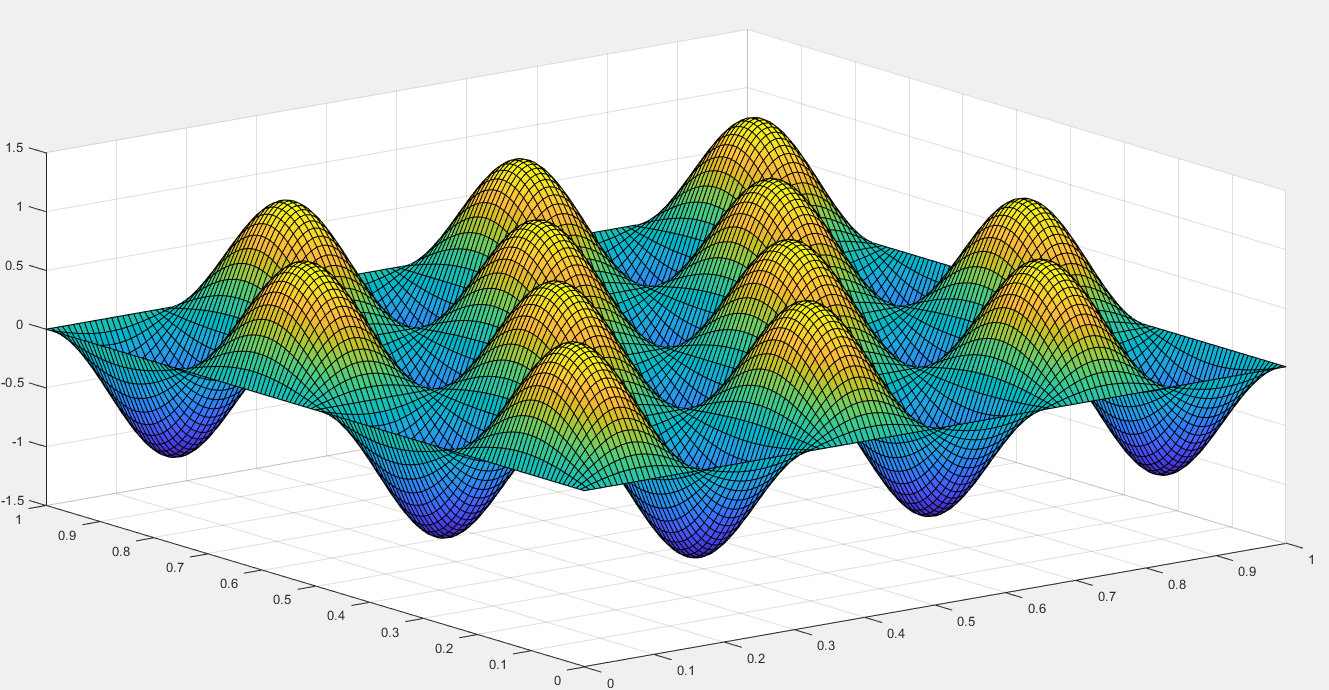
\includegraphics[width=\linewidth]{Aufgaben-Ressourcen/A6L7M3N2.png}
		\caption{Poisson-Problem: Lösung}
\end{figure}

Implementierung: Linksvorkonditioniertes GMRES-Verfahren\\
Vergleichsimplementierung: GMRES-Verfahren\\
Das vorkonditionierte Verfahren konvergiert schneller als das gewöhnliche GMRES-Verfahren. Allerdings ist die Laufzeit trotzdem je nach der gewählten Genauigkeit langsamer als im gewöhnlichen GMRES. Dies liegt daran, dass die Bestimmung des Vorkonditionierers am Anfang und dessen Anwendung in jeder Iteration die Laufzeit verlängert. Mit l=5 gilt, wenn der globale Fehler kleiner als 0.8*10$^{-5}$ ist ist die vorkonditionierte Version schneller. Dieser Fehlergrenzwert erhöht sich mit der Erhöhung von l.\\
Die Messungen wurden mit l=5 M=3 N=2 und variierender Fehlerschranke f durchgeführt. Die Messwerte können in Table \ref{Table:2_4d} abgelesen werden. In den Datenzellen steht jeweils die Anzahl der Iterationen und durch ein Simikolon getrennt die Laufzeit in Sekunden.\\
\begin{table}
\begin{tabular}{|l|l|l|r|r|r|}
	\hline
	Algorithmus&f=$10^{-5}$ &$10^{-6}$&$9*10^{-7}$& $8*10^{-7}$& $7*10^{-7}$\\
	\hline
	GMRES & 33;0.423 & 173;1.181 & 213;1.378 & 269;1.953 & 351;2.683 \\
	Vorkonditioniert & 18;0.725 & 21;1.760 & 29;1.921 & 36;2.111 & 36;2.106 \\
	\hline
	
\end{tabular}
	\caption{Vergleich zwischen GMRES und vorkonditioniertem GMRES}
	\label{Table:2_4d}
\end{table}
\section{Heizprozesssimulation einer Herdplatte}
\subsection{Aufgabe 5}

\subsubsection{Mathematische Grundlage}
Im folgenden Abschnitt werden folgende Funktionen und Parameter verwendet:\\
u(t$_{n}$) := Wärme an allen räumlichen Diskretisierungspunkten zum Zeitpunkt t$_{n}$\\
u'(t$_{n}$) := Wärmeänderungen an allen räumlichen Diskretisierungspunkten zum Zeitpunkt t$_{n}$\\
u$_{i,j}$(t$_{n}$) := Wärme am räumlichen Diskretisierungsschritt (i,j) zum Zeitpunkt t$_{n}$\\
u'$_{i,j}$(t$_{n}$) := Wärmeänderungen am räumlichen Diskretisierungsschritt (i,j) zum Zeitpunkt t$_{n}$\\
u(x,y,t$_{n}$) := Wärme am räumlichen Punkt (x,y) zum Zeitpunkt t$_{n}$\\
u'(x,y,t$_{n}$) := Wärmeänderungen am Punkt (x,y) zum Zeitpunkt t$_{n}$\\
f := Heizfunktion an allen räumlichen Diskretisierungspunkten (zeitlich invariant) $f(x,y) = 32 * [x*(x-1)+y*(y-1)]$\\
h$_{t}$ := Zeitlicher Diskretisierungsparameter (Zeitschrittweite)\\
h$_{s}$ := Räumlicher Diskretisierungsparameter (Schrittweite zwischen den räumlichen Diskretisierungspunkten)\\
a := Temperaturleitfähigkeit des Materials \\
A := Matrix mit besonderer Struktur für Finite Differenzen\\
t$_{n}$ := Zeitpunkt nach n Zeitschritten\\
t$_{0}$ := Startzeitpunkt\\
N := Menge der natürlichen Zahlen\\
\\
Wir benutzen die nicht homogene Wärmeleitungsgleichung, da wir nicht nur die Wärmeverteilung simulieren wollen, sondern mit der Funktion f Wärme hinzugefügt werden soll. Damit lautet die Gleichung:\\
\\
$u'(t) - a * \triangle u(t) = f$\\
\\
Damit unser Modellproblem korrekt gestellt ist definieren wir folgendes:\\
\\
$- \triangle u(x,y,t_{n}) = \frac{f(x,y)-u'(x,y,t_{n})}{a}   ,$   $  (x,y) \in \Omega = (0,1)^2  ,$   $  n \in N\backslash0;$\\
$u(x,y,t_{n}) = 20,$   $(x,y) \in \Gamma ,$   $ n \in N;$\\
$u(x,y,t_{0}) = 20,$   $ (x,y) \in \Omega ; $ \\
f(x,y) ist stetig,   $ (x,y) \in \Omega .$ \\
\\
Damit sind unsere Rand- und Anfangsbedingungen gesetzt. Wir haben also u(t$_{0}$) gegeben und kennen f. Damit können wir u'(t$_{0}$) bestimmen indem wir unsere Basisgleichung umstellen.\\
\\
$u'(t_{n})  = f + a * \triangle u(t_{n})$\\
mit $\triangle u(t_{n}) = \frac{4*u_{i,j}(t_{n})-u_{i-1,j}(t_{n})-u_{i+1,j}(t_{n})-u_{i,j-1}(t_{n})-u_{i,j+1}(t_{n})}{h_{s}^{2}}$\\
\\
Im Fall von unserem $u(t_{0})$ ist $\triangle u(t_{n})$ = 0, da es keine Hitzeunterschiede in $u(t_{0})$ gibt. Anschließend können wir $u(t_{1})$ bestimmen und damit den Zeitschritt volziehen. Dafür eignet sich das explizite Eulerverfahren und als Gleichung ergibt sich:\\
\\
$u(t_{n+1})  =u(t_{n}) + h_{t} * u'(t_{n})$\\
\\
Nun haben wir alles um das Poissonproblem zu lösen. Die oben definierte Gleichung konvertieren wir um sie numerisch zu lösen. Da wir u' von unserem neuen Zeitschritt noch nicht kennen ersetzen wir es durch $\frac{ u(t_{n}) -  u(t_{n-1})}{h_{t}}$.\\
\\
$A* u(t_{n}) = \frac{h_{s}^{2}}{a} * ( f-\frac{ u(t_{n}) -  u(t_{n-1})}{h_{t}}) $\\
\\
Die Lösung des Problems gibt uns u(t$_{1}$) und dadurch können wir wieder mit dem ersten Schritt weiter machen. Damit lässt sich jeder beliebige Zeitschritt berechnen.
\subsubsection{Implementierung}
Wir haben uns für die Implentierung des Poisson-Gleichungs-Lösers für einen vorkonditionierten GMRES-Algorithmus entschieden, da die Matrix A konstant bleibt und man somit den Vorkonditionierer nur ein Mal bestimmen muss und trotzdem in jeder Iteration davon profitiert. Wir haben a=1 angenommen in unserer Implementierung und alle anderen Parameter sind konfigurierbar. Außerdem werden die Hitzedaten in jedem x-ten Zeitschritt ausgegeben, wobei man x frei wählen kann. Bei den Zeitschritten 5, 30 und 60 ergeben sich die in den Grafiken dargestellten Hitzewerte. \\

\begin{figure}
	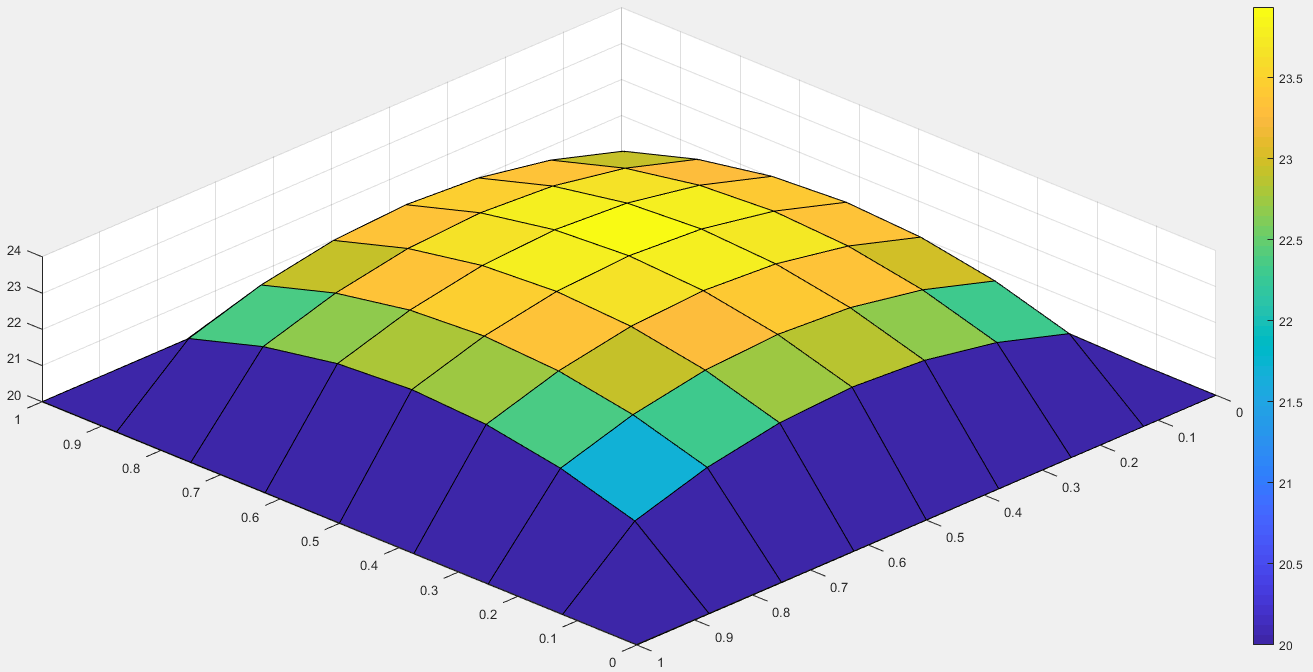
\includegraphics[width=\linewidth]{Aufgaben-Ressourcen/P2A5T5.png}
		\caption{u($t_{5})$}
\end{figure}
\begin{figure}
	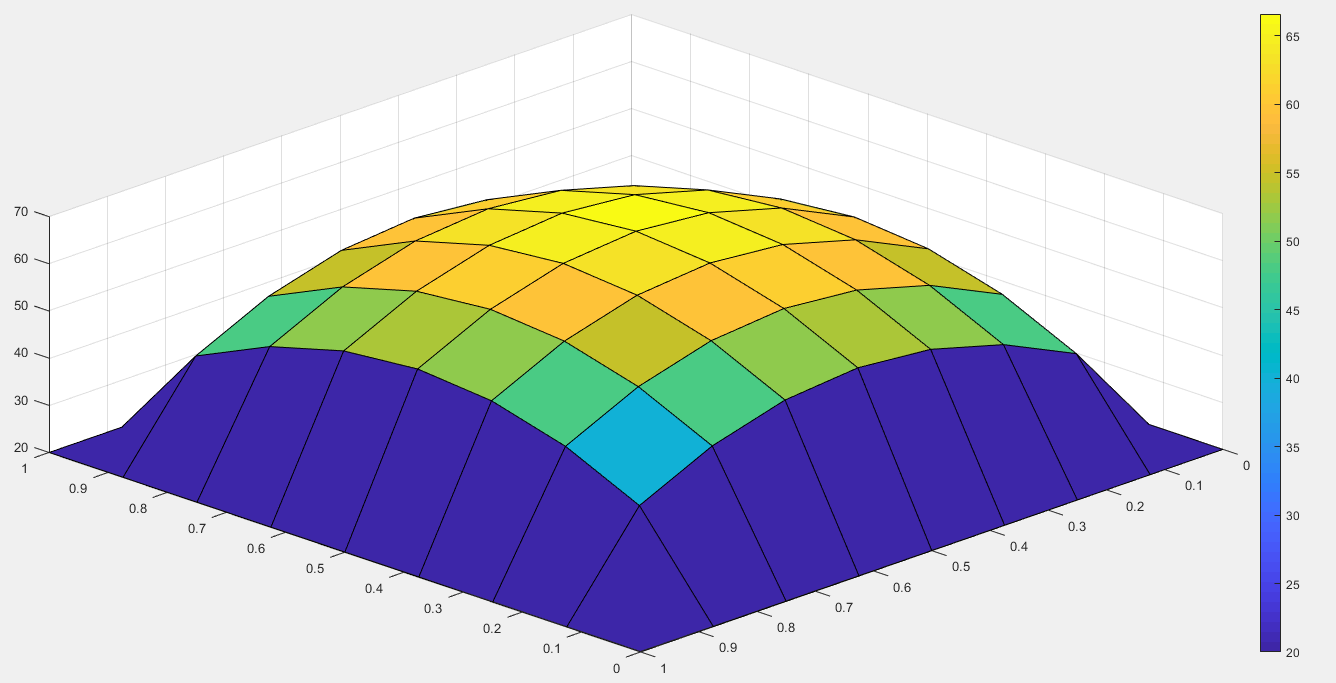
\includegraphics[width=\linewidth]{Aufgaben-Ressourcen/P2A5T30.png}
		\caption{u($t_{30})$}
\end{figure}
\begin{figure}
	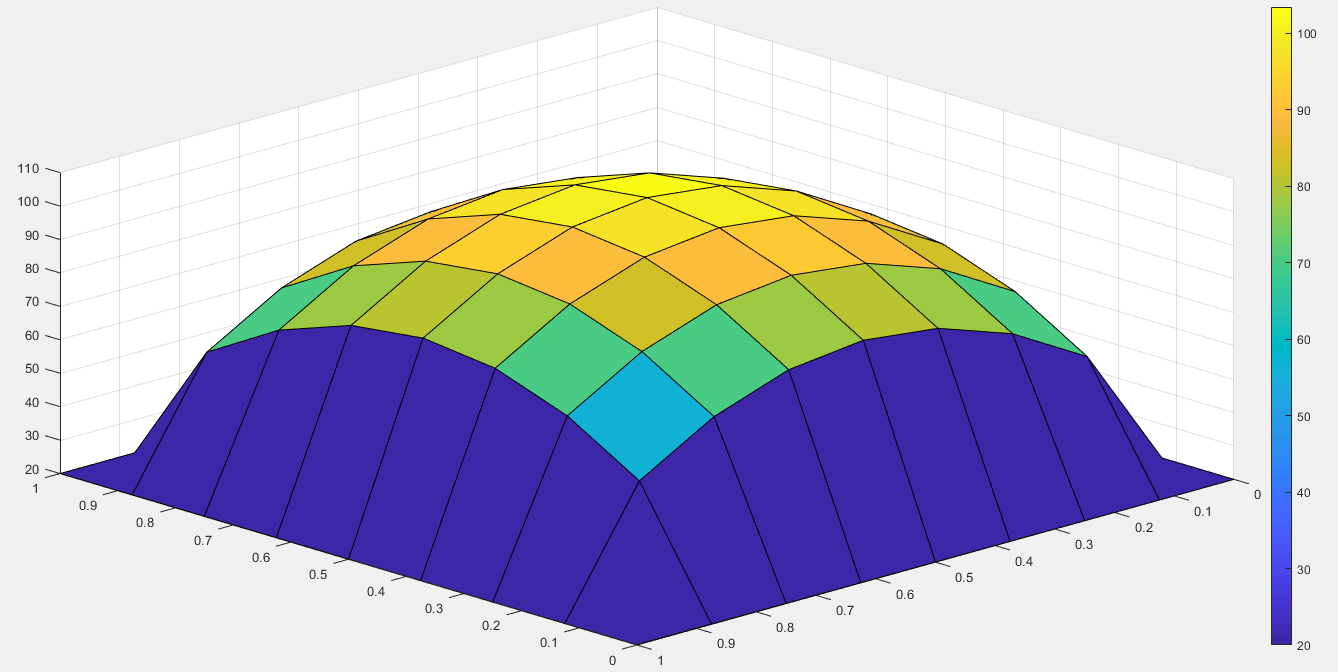
\includegraphics[width=\linewidth]{Aufgaben-Ressourcen/P2A5T60.png}
		\caption{u($t_{60})$}
\end{figure}


	


\end{document}
